\section*{\begin{center}{\Huge Appendix}\end{center}}
\addcontentsline{toc}{chapter}{Appendix}
$\\[0.5cm]$

\noindent Write your appendix here...

\todo[inline]{Include confusion matrices for the remaining data sets}
 
\section{Additional Results}

\subsection{Measuring error rate}

\begin{table}[H]
	\centering
	\begin{tabular}{|l|l|l|l|}
		{\bf Experiment Name}            & {\bf Mean error} & {\bf Std. dev.} & {\bf $\lambda$} \\
		\hline
		Centralized logistic regression  & $0.104$          & $0.0059$        & $2^{-8}$        \\
		Disjoint logistic regression     & $0.159$          & $0.0026$        & $2^{-5}$        \\
		Aggregated model, $\epsilon=1.0$ & $0.163$          & $0.0103$        & $2^{-3}$        \\
		Ensemble model, $\epsilon=1.0$   & $0.150$          & $0.0045$        & $2^{-5}$        \\
		Aggregated model, $\epsilon=0.1$ & $0.182$          & $0.0256$        & $2^{-1}$        \\
		Ensemble model, $\epsilon=0.1$   & $0.157$          & $0.0117$        & $2^{-2}$       
	\end{tabular}
	\caption{Measuring accuracy: Spambase}
	\label{tab:results_measuring_accuracy_spam}
\end{table}


\begin{table}[H]
	\centering
	\begin{tabular}{|l|l|l|l|}
		{\bf Experiment Name}            & {\bf Mean error} & {\bf Std. dev.} & {\bf $\lambda$} \\
		\hline
		Centralized logistic regression  & 0.306            & 0.0809          & $2^{2}$         \\
		Disjoint logistic regression     & 0.279            & 0.0035          & $2^{-3}$        \\
		Aggregated model, $\epsilon=1.0$ & 0.271            & 0.0056          & $2^{-2}$        \\
		Ensemble model, $\epsilon=1.0$   & 0.274            & 0.0034          & $2^{-3}$        \\
		Aggregated model, $\epsilon=0.1$ & 0.291            & 0.0112          & $2^0$           \\
		Ensemble model, $\epsilon=0.1$   & 0.285            & 0.0087          & $2^0$          
	\end{tabular}
	\caption{Measuring accuracy: Susy}
	\label{tab:results_measuring_accuracy_susy}
\end{table}

\begin{table}[h]
	\centering
	\begin{tabular}{llll}
		& \multicolumn{3}{c}{Actual}                                                      \\
		\multicolumn{1}{c}{} &                        & 1                         & 0                          \\ \cline{3-4} 
		Predicted            & \multicolumn{1}{l|}{1} & \multicolumn{1}{l|}{273} & \multicolumn{1}{l|}{49}   \\ \cline{3-4} 
		& \multicolumn{1}{l|}{0} & \multicolumn{1}{l|}{81} & \multicolumn{1}{l|}{518} \\ \cline{3-4} 
	\end{tabular}
	\caption{Confusion Matrix: Spambase. Local model only.}
	\label{fig:confmat_spam_local}
\end{table}

\begin{table}[h]
	\centering
	\begin{tabular}{llll}
		& \multicolumn{3}{c}{Actual}                                                      \\
		\multicolumn{1}{c}{} &                        & 1                         & 0                          \\ \cline{3-4} 
		Predicted            & \multicolumn{1}{l|}{1} & \multicolumn{1}{l|}{268} & \multicolumn{1}{l|}{38}   \\ \cline{3-4} 
		& \multicolumn{1}{l|}{0} & \multicolumn{1}{l|}{86} & \multicolumn{1}{l|}{529} \\ \cline{3-4} 
	\end{tabular}
	\caption{Confusion Matrix: Spambase. Aggregated, DP model only.}
	\label{fig:confmat_spam_aggdp}
\end{table}

\begin{table}[h]
	\centering
	\begin{tabular}{llll}
		& \multicolumn{3}{c}{Actual} \\
		\multicolumn{1}{c}{} &                        & 1                         & 0                          \\ \cline{3-4} 
		Predicted            & \multicolumn{1}{l|}{1} & \multicolumn{1}{l|}{257} & \multicolumn{1}{l|}{35}   \\ \cline{3-4} 
		& \multicolumn{1}{l|}{0} & \multicolumn{1}{l|}{97} & \multicolumn{1}{l|}{5d32} \\ \cline{3-4} 
	\end{tabular}
	\caption{Confusion Matrix: Spambase. Ensemble of Aggregated and Local.}
	\label{fig:confmat_spamd_ensemble}
\end{table}

\subsection{Changes in number of participants}


\begin{figure}[H]
	\centering
	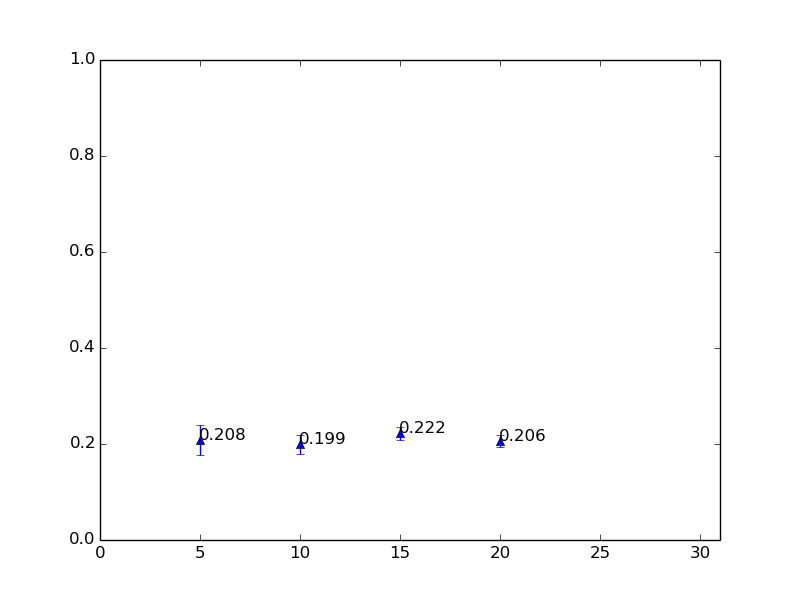
\includegraphics[width=\textwidth]{fig/spambase/eps1.0,bud1.0,peers5-30,groups5,reg2e-2-puball-peercounts-data150-spam-testmean}
	\caption{Effect of peer numbers. Spambase.}
	\label{fig:peer_range_constant_group_spam}
\end{figure}


\subsection{Peer error rate variance}

\begin{table}[H]
	\centering
	
	\begin{tabular}{|l|l|l|}
		\textbf{Model}                  & \textbf{Mean error} & \textbf{Peer std. dev.} \\
		\hline
		Local, no privacy      & 0,159 & 0.016 \\
		Aggregated, d. privacy & 0,163 & 0.000	 \\
		Ensemble with both & 0.150 & 0.006 \\
	\end{tabular}
	\caption{Variance among peers. Spambase.}
	\label{table:peer_variance_spam}
\end{table}

Note that the results seen in Table \ref{table:peer_variance_spam} differ in the experimental setup described Section \ref{sec:experiment_peer_variance} in that each peer had 300 records instead of 250.

\subsection{Effect of aggregation group size and model propagation}


\begin{table}[H]
	\centering
	\begin{tabular}{|l|l|l|l|}
		{\bf \begin{tabular}[c]{@{}l@{}}Group \\ size\end{tabular}} & {\bf \begin{tabular}[c]{@{}l@{}}Mean \\ error\end{tabular}} & {\bf \begin{tabular}[c]{@{}l@{}}Error\\ std. dev.\end{tabular}} & {\bf \begin{tabular}[c]{@{}l@{}}Peer error\\ std. dev.\end{tabular}} \\
		\hline
		1                                                           & 0.233                                                       & 0.0184                                                          & 0.0435                                                               \\
		5                                                           & 0.217                                                       & 0.0185                                                          & 0.0399                                                               \\
		10                                                          & 0.223                                                       & 0.0179                                                          & 0.0368                                                               \\
		15                                                          & 0.221                                                       & 0.0245                                                          & 0.0290                                                               \\
		20                                                          & 0.205                                                       & 0.0323                                                          & 0.0257                                                              
	\end{tabular}
	\caption{Effect of aggregation group size. Party-publishing. Spambase.}
	\label{tab:results_groupsize_party_spam}
\end{table}

\begin{table}[H]
	\centering
	\begin{tabular}{|l|l|l|l|}
		{\bf \begin{tabular}[c]{@{}l@{}}Group \\ size\end{tabular}} & {\bf \begin{tabular}[c]{@{}l@{}}Mean \\ error\end{tabular}} & {\bf \begin{tabular}[c]{@{}l@{}}Error\\ std. dev.\end{tabular}} & {\bf \begin{tabular}[c]{@{}l@{}}Peer error\\ std. dev.\end{tabular}} \\
		\hline
		1                                                           & 0.215                                                       & 0.0076                                                          & 0.0036                                                               \\
		5                                                           & 0.211                                                       & 0.0135                                                          & 0.0125                                                               \\
		10                                                          & 0.197                                                       & 0.0116                                                          & 0.0191                                                               \\
		15                                                          & 0.200                                                       & 0.0090                                                          & 0.0225                                                               \\
		20                                                          & 0.195                                                       & 0.0110                                                          & 0.0202                                                              
	\end{tabular}
	\caption{Effect of aggregation group size. All-publishing. Spambase.}
	\label{tab:results_groupsize_all_spam}
\end{table}

\subsection{Value of budgeting privacy}

\begin{figure}[H]
	\centering
	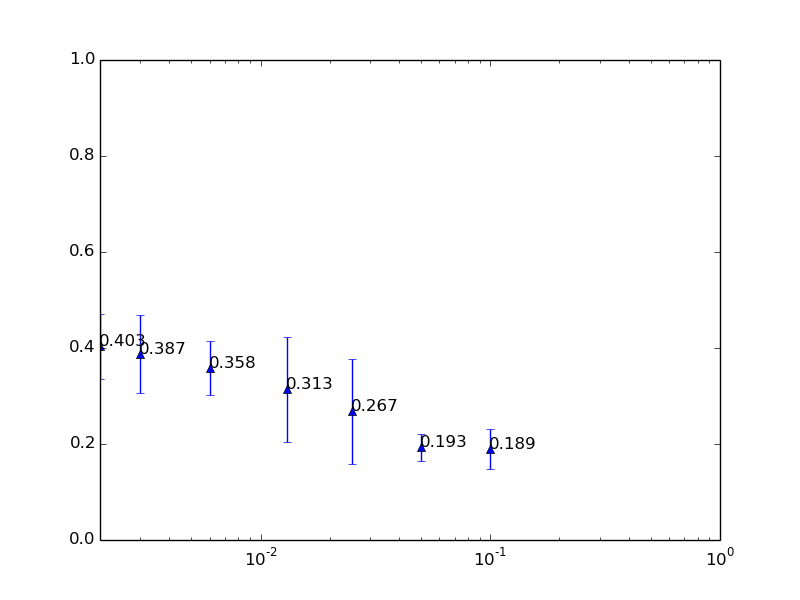
\includegraphics[width=.8\textwidth]{fig/spambase/eps0.1,buddiv1-64,peers10,groups5,reg2e-2-puball-budgeting-data300-spam-testmean}
	\caption{Effect of Privacy Budgeting. Spambase.}
	\label{fig:results_privacy_budget_spam}
\end{figure}